% !TeX root = ../apuntes-ea.tex

\chapter{Anillos. Cuerpos}

\newcommand{\0}{\mathbf{0}}
\newcommand{\1}{\mathbf{1}}

En este capítulo se extiende lo que sabemos de teoría de grupos a las nuevas estructuras algebraicas que introducimos que son los anillos y los cuerpos.

\section{Definición y propiedades básicas}

\begin{dfn}[Anillo]
	Un anillo es una terna $(A, +, \cdot)$ donde $+: A \times A \to A$ es una operación a la que llamamos suma, $\cdot: A \times A \to A$ es otra operación a la que llamamos producto y se verifican las siguientes propiedades
	\begin{enumerate}
		\item El par $(A, +)$ es un grupo abeliano
		\item El producto $\cdot$ es asociativo
		\item Se cumplen las propiedades distributivas:
		\begin{align}
			\forall a, b , c \in A,\ a\cdot (b + c) = a\cdot b + a \cdot c \\
			\forall a, b , c \in A,\ (a + b) \cdot c = a\cdot c + b \cdot c
		\end{align}
	\end{enumerate}
\end{dfn}

Con la operación $+$ tenemos las siguientes propiedades
\begin{enumerate}
	\item Asociatividad: $(a+b)+c = a+(b+c)$
	\item Elemento neutro aditivo: $\exists! \0 \in A \mid \0+a = a$
	\item Elemento inverso aditivo: $\forall a \in A, \exists -a \in A \mid a + (-a) = \0$
	\item Conmutatividad aditiva: $\forall a, b \in A,\ a+b = b+a$
\end{enumerate}

Con la operación $\cdot$ tenemos las siguientes propiedades
\begin{enumerate}
	\item Asociatividad: $a\cdot (b \cdot c) = (a \cdot b) \cdot c$
	\item No siempre existe el neutro multiplicativo: $\1 \in A \mid a\cdot 1 = 1 \cdot a = a$
	\item No siempre el producto es conmutativo.
	\item No siempre existe inverso multiplicativo: $\inv{a} \mid a\cdot \inv{a} = \1$
	\item No siembre se da la conmutatividad multiplicativa: $a \cdot b = b\cdot a$
\end{enumerate}

\begin{pro}
	$\forall a \in A,\ a\cdot \0 = \0$
\end{pro}

\begin{proof}
	$a \cdot \0 = a \cdot(\0 + \0) = a\cdot \0 + a\cdot \0 \implies \0 = a\cdot \0$
\end{proof}

\begin{dfn}[Anillo con unidad]
	Sea $(A, +, \cdot)$ un anillo. Decimos que es un anillo con unidad si $\exists \1 \in A \mid \forall a \in A, \1 a = a \1 = a$.
\end{dfn}

\begin{pro}
	El neutro multiplicativo, $\1$, si existe, es único.
\end{pro}

\begin{dfn}[Anillo conmutativo]
	Sea $(A, +, \cdot)$ un anillo. $A$ es un anillo conmutativo $\iff \forall a, b \in A,\ a\cdot b = b \cdot a$.
\end{dfn}

\begin{pro}
	Sea $(A, +, \cdot)$ un anillo con más de un elemento ($|A| > 1$). Entonces $\0 \neq \1$ (el neutro aditivo es distinto del neutro multiplicativo).
\end{pro}

\begin{proof}
	Por contradicción. Sea $a \neq \0 \in A$ y $\0 = \1$. Entonces $a = a\cdot \1 = a\cdot 0 = 0 \implies a = \0$ contradicción.
\end{proof}

Para acabar veamos algunos ejemplos.

\begin{ej}
	Las matrices cuadradas $2\times 2$ con coeficientes reales: $(M_{2\times 2}(\R), +, \cdot)$ es un anillo con unidad ($\1 = I$) pero no es conmutativo. Tiene unidades $\uds{A} = (GL_2(\R), \cdot)$
\end{ej}

\begin{ej}
	Es cierto que $\Z, \mathbb{Q}, \R, \mathbb{C}$ son anillos con unidad con las operaciones suma y producto habituales. Además hay otros como por ejemplo $\Z[i] = \{a+bi \in \mathbb{C} \mid a,b \in \Z\}$. Son todos conmutativos porque el producto en estos conjuntos es conmutativo.
\end{ej}


\subsection{Unidades en anillos}

Además, para pulir lo de que no siempre existe inverso multiplicativo daremos la definición de Grupo de unidades en el contexto de anillos que da sentido al \autoref{ej:grupounidades} que hemos estado utilizando.

\begin{dfn}[Unidades en anillos]
	Dado $(A, +, \cdot)$ anillo. El grupo de unidades es
	\begin{align}
		\uds{A} = (\{a \in A \mid \exists \inv{a} \in A,\ a\cdot \inv{a} = \1\}, \cdot)
	\end{align}
	Los elementos del grupo de unidades se llaman \textbf{elementos invertibles}.
\end{dfn}

Para que este grupo quede bien definido estaría bien que $\inv{a}$ fuera único.

\begin{pro}
	El inverso multiplicativo es único.
\end{pro}

\begin{proof}
	Sea $a \in A$. Supongamos $a', a'' \in A$ son ambos inversos multiplicativos de $a$:
	\begin{align*}
		aa' = \1 \land aa'' = \1\implies \begin{cases}
		a''(aa') = a'' \\
		(a''a)a' = a''
		\end{cases}\implies a' = a''
	\end{align*}
\end{proof}

\begin{pro}
	Sea $-\1$ el inverso aditivo del neutro multiplicativo $\1$. Entonces $\forall a \in A$ el inverso aditivo es $-a = -\1 \cdot a$ y se tiene $-\1\cdot a + a = 0$.
\end{pro}

\begin{pro}
	Sea $A$ un anillo. El neutro aditivo $\0$ verifica $\0 \not\in \uds{A}$
\end{pro}

\begin{pro}[Propiedad cancelativa]
	Sea $a \in \uds{A}$. Entonces $\forall b,c$ se tiene $b, c \in A \implies a\cdot b = a\cdot c \implies b = c$
\end{pro}

\begin{pro}
	$a \in \uds{A} \iff \gen{a} = A$
\end{pro}

\begin{proof}$ $\newline
	\begin{enumerate}
		\item $(\implies)\qquad a \in \uds{A} \implies \exists \inv{a} \implies \gen{a} = A\cdot a = \{\alpha a \mid \alpha \in A\}$. Si $a \in \uds{A} \implies \exists \inv{a} \implies \inv{a}a = \1 \in \gen{a} \iff \gen{a} = A$
		
		\item $(\impliedby$) Si $\gen{a} = A$ entonces $\exists b \in A \mid ba = \1 \implies b = \inv{a} \implies a \in \uds{A}$.
	\end{enumerate}
\end{proof}

\begin{ej}
	Los numeros enteros $(\Z, +, \cdot)$ es un anillo y tienen unidades $\uds{\Z} = (\{-1, 1\}, \cdot)$
\end{ej}

\section{Subanillos}

La siguiente definición es de \cite{dor96}:

\begin{dfn}[Subanillo]
	Sea $(A, +, \cdot)$ un anillo, $B\subset A$. Decimos que $B$ es un subanillo si $(B, +)$ es subgrupo de  $(A, +)$ y el producto restringido a $B$ es cerrado.
\end{dfn}

La definición que ha dado Orlando es algo diferente. Es equivalente a la anterior y la plasmamos como una proposición.

\begin{pro}
	$B \subset A$ es un subanillo si ambas operaciones son cerradas y $(B, +, \cdot)$ es un anillo (tiene la estructura de anillo).
\end{pro}

\begin{ej}
	$(\Z, +, \cdot)$ es un subanillo de $(\Q, +, \cdot)$.
\end{ej}



\section{Dominios de integridad.}

\begin{dfn}[Divisor de 0]
	Sea $(A, +, \cdot)$ un anillo. Diremos que $a \in A$ es divisor de $\0 \iff a \neq \0 \land \exists b \neq \0 \in A \mid a\cdot b = \0$
\end{dfn}

\begin{ej}
	En $\Z/8\Z$ el elemento $\overline{2}$ es un divisor de $\0$:
	\begin{align*}
		\overline{2}\cdot\overline{4} = \overline{8} = \0
	\end{align*}
	Sin embargo, $\overline{3}$ no lo es ya que
	\begin{align*}
		\overline{3}\overline{a} = \0 \implies \inv{\overline{3}}\overline{3}\overline{a} = \inv{\overline{3}}\0 \implies \1 \overline{a} = \0 \implies \overline{a} = 0
	\end{align*}
\end{ej}

Otra manera de ver esto es plantear la ecuación $a \cdot b = \0$. El $\0$ siempre es una solución, pero podemos decir que $a$ es un divisor de $\0$ si la ecuación tiene soluciones no triviales.

\begin{ej}$ $\newline
	\begin{itemize}
		\item En $\Z$ la ec. $2x = 0$ solo tiene la solución trivial $\implies 2$ no es un divisor de $\0$.
		\item En $\Z/6\Z$ la ec. $\overline{2}\overline{x} = 0$ tiene la solución $\overline{x} = \overline{3}$ luego $\overline{2}$ sí que es un divisor de $0$.
	\end{itemize}
\end{ej}

\begin{pro}
	Si $a \in \uds{A}$ entonces $a$ no es un divisor de $0$.
\end{pro}

\begin{proof}
	Si $a \in \uds{A}$ sabemos que existe $\inv{a} \mid \inv{a}a = \1 \implies ax = \0 \iff \inv{a}ax = \inv{a} \0 \iff \1 x = \0 \iff x = \0$ luego la ecuación solo tiene la solución trivial.
\end{proof}

\begin{pro}
	Sea $A$ un anillo. $\forall a \in A$ no divisor de 0 $\implies$ se cumple la propiedad cancelativa.
\end{pro}

\begin{proof}
	$ab = ac \implies b = c \iff ab + (-ac) = a(b -c) = \0$
\end{proof}

\begin{dfn}[Dominio de integridad]
	Un anillo que no tiene elementos divisores de 0 se llama dominio de integridad (DI).
\end{dfn}

% TODO profundizar con la p. 159 de santorum
\begin{ej}$ $\newline
	\begin{itemize}
		\item $\Z$ es un dominio de integridad ya que todo $a \in \Z, a \neq \0$ tiene un inverso multiplicativo $\inv{a}$.
		\item $\Z/p\Z$ con $p$ primo es un dominio de integridad.
		\item $\Z/n\Z$ con $n$ no primo no es un dominio de integridad ya que si $\overline n = ab$ con $a \neq n \land b \neq n$ se tiene $\overline{a} \cdot \overline{b} = \overline{n} = \0$ con $\overline{a} \neq \0 \land \overline{b} \neq \0$.
	\end{itemize}
\end{ej}


Es tan memorable la siguiente proposición que a veces la utilizamos como definición de dominio de integridad.

\begin{pro}
	$A$ es un DI $\iff$ el producto de elementos no nulos es no nulo.
\end{pro}

\begin{proof}
	$(\impliedby)$ Sean $a,b \in A,\ a,b \neq \0 \implies ab \neq 0 \implies A$ dominio de integridad.
	
	$(\implies)$ Sea $a \in A,\ a \neq \0$. $A$ DI $\implies \nexists b \in A \mid a\cdot b = \0 \iff$ el producto de no nulos es no nulo.
\end{proof}


\section{Cuerpos}

\begin{dfn}[Cuerpo]
	Diremos que un anillo con unidad es un cuerpo si $\uds{A} = A \setminus \{\0\}$
\end{dfn}

Esto quiere decir que un anillo es un cuerpo si todo elemento a excepción del $\0$ tiene inverso multiplicativo.

\begin{ej}
	\item $\Z/p\Z$ con $p$ primo es un cuerpo
	\item $\Z$ o $\Z/6\Z$ no son cuerpos
	\item $\Q$ es un cuerpo (es el primero que sale al ir añadiendo números a los naturales)
	\item $\R$ y $\mathbb{C}$ también son cuerpos
	\item Las matrices $2 \times 2$ invertibles que antes veíamos como un grupo solo con el producto también son un cuerpo si les añadimos la suma: $(GL_2(\R), +, \cdot)$ es un cuerpo.
\end{ej}

\begin{pro}
	Sea $(A, +, \cdot)$ un anillo. Son equivalentes:
	\begin{enumerate}
		\item $A$ es un cuerpo
		\item El retículo de ideales es el normal
	\end{enumerate}
\end{pro}

\begin{pro}
	Si $A$ es un cuerpo entonces $A$ es un DI.
\end{pro}


Hay que buscar una buena definición para esto.
\begin{dfn}[Estructura de anillos]
	% TODO: dar una definición de verdad
	Sea $(A, +, \cdot)$ un anillo. Una estructura de anillos $A[x]$ es una cosa con elementos de la forma $ax$ para $a \in A$.
\end{dfn}

\begin{pro}
	$A$ DI $\implies A[x]$ DI
\end{pro}

\begin{obs}
	NO se da el recíproco: por ejemplo, $\Q$ es un cuerpo $\implies \Q$ DI $\implies \Q[x]$ dominio, PERO $\Q[x]$ no es un cuerpo.
\end{obs}

\section{Homomorfismos de anillos}

Cuando vimos los grupos, esperamos un poco más para hablar de homomorfismos. Aquí no lo haremos ya que solo necesitamos extender la definición.

\begin{dfn}[Homomorfismo de anillos]
	Sean $(A, +, \cdot), (B, \oplus, \odot)$ anillos y sea $\varphi: A \to B$. Decimos que $\varphi$ es un homomorfismo de anillos si
	\begin{enumerate}
		\item $\varphi(a_1+a_2) = \varphi(a_1) \oplus \varphi(a_2)$
		\item $\varphi(a_1 \cdot a_2) = \varphi(a_1)\odot\varphi(a_2)$
		\item $\varphi(\1_A) = \1_B$
	\end{enumerate}
\end{dfn}

\begin{obs}
	Dado $\varphi:A \to B$ homomorfismo de anillos, $\ima \varphi \subset B$ siempre es un subanillo de $B$.
\end{obs}

\begin{pro}[Inyectividad/sobreyectividad en homomorfismos de anillos]
	Sea $\varphi: A \to B$ un homomorfismo de anillos.
	\begin{itemize}
		\item $\varphi$ inyectivo $\iff \ker \varphi = \{\0\}$
		\item $\varphi$ sobre $\iff \ima \varphi = B$
	\end{itemize}
\end{pro}

\begin{pro}
	El homomorfismo de anillos $\varphi: A \to B$ es una biyección de conjuntos $\iff \ker \varphi = \{\0\} \land \ima \varphi = B$.
\end{pro}

\begin{obs}
	Si $\varphi:A \to B$ homomorfismo de anillos es una biyección de conjuntos entonces $\inv{\varphi}:B \to A$ también es un homomorfismo de anilos.
\end{obs}

\begin{dfn}[Isomorfismo de anillos]
	Diremos que un homomorfismo de anillos $\varphi:A \to B$ es un isomorfismo de anillos $\iff \exists \inv{\varphi} : B \to A$ tal que
	\begin{align*}
	\varphi \circ \inv{\varphi} = Id_B \land \inv{\varphi} \circ \varphi = Id_A
	\end{align*}
\end{dfn}

\begin{pro}
	Sea $\varphi:A \to B$ un homomorfismo de anillos. Entonces $\varphi$ es un isomorfismo de anillos $\iff \ker \varphi = \{\0\} \land \ima \varphi = B$.
\end{pro}

\section{Ideales}

La definición de ideal se puede dar de dos maneras. Así la ha dado Orlando:

\begin{dfn}[Ideal]
	Un subconjunto $I \subset A$ es un ideal $\iff$
	\begin{enumerate}
		\item $\0 \in I$
		\item $s,t \in I \implies s+t \in I$
		\item $s \in I \land a \in A \implies a \cdot s \in I \land s \cdot a \in I$
	\end{enumerate}
\end{dfn}

Esta es otra definición alternativa:

\begin{dfn}[Ideal (alternativa)]
	Sea $I$ un subanillo de $A$. Decimos que $I$ es un ideal $\iff \forall i \in I, \forall a \in A,\ ai \in I \land ia \in A$.
\end{dfn}

\begin{pro}
	Si $I$ es un ideal en $A$ entonces $(I, +) < A$ (es decir, $I$ es un subgrupo aditivo de $A$).
\end{pro}

\begin{pro}
	Sea $I \subset A$ un ideal. Entonces $\1 \in I \iff I = A$.
\end{pro}

\begin{proof}
	Por la tercera propiedad de los ideales tenemos que $\1 \in I \implies \forall a \in A,\ \1 \cdot a \in I \implies A \subseteq A \implies A = I$.
	
	El otro sentido es trivial.
\end{proof}

\begin{ej}
	$0\Z,\ 1\Z,\ 2\Z, 3\Z,\ 4\Z$ son todos ideales de $\Z$ (y subgrupos de $(\Z, +)$).
\end{ej}

\begin{pro}
	Sea $\{I_j\}_{j \in J}$ una familia de ideales en $A$ ($I_j \subset A$ es un ideal para cada $j \in J$). Entonces $\cap_{j \in J} I_j$ es un ideal en $A$.
\end{pro}

\begin{ej}
	En el anillo $\Z$ están los ideales $6\Z$ y $8\Z$. Por la proposición anterior $6\Z \cap 8\Z$ es un ideal (es $mcd(6,8)\Z = 2\Z$).
\end{ej}

\begin{pro}
	Sean $I, J \subset A$ ideales. Entonces $I + J = \{i + j \mid i \in I \land j \in J\}$ es un ideal\footnote{Ojo: aquí $I+J$ no tiene nada que ver con la suma directa (el caso particular del producto directo) que había en grupos.} de $A$ que contiene a $I$, a $J$, y además es el mayor ideal con esta propiedad.
\end{pro}

A continuación definimos el análogo al subgrupo generado pero para anillos:

\begin{dfn}[Ideal generado por un subconjunto]
	De \cite{dor96}. Sea $(A, +, \cdot$ un anillo, $S \subset A$. Definimos el ideal generado por $S$ y lo denotamos con $\gen{S}$ como el conjunto de todas las palabras de longitud $n$ en los elementos de $S$, para $n \in \N$. Esto es:
	\begin{align*}
		\gen{S} = \{s_1\cdot a_1 + \dots + s_na_n \mid a_i \in A,\ s_i \in S, n \in \N\} = \{\sum_{i=1}^{n} a_is_i \mid a_i \in A,\ s_i \in S, n \in \N\}
	\end{align*}
\end{dfn}

Ojo al abuso de notación en la definición anterior. El sumatorio y el producto implícito hacen referencia a las operaciones definidas en el anillo $(A, +, \cdot)$.

Como cabe esperar, cumple las mismas propiedades que cumplían los subgrupos generados.

\begin{pro}
	Sea $S = \{S_1, \dots, S_r\} \subset A$ y sea $\gen{S} = \{\sum_{i=1}^{r}a_is_i \mid a_i \in A\}$. Entonces
	\begin{enumerate}
		\item $\gen{S}$ es un ideal\footnote{Es para asegurarnos de que la construcción que hemos dado produce un ideal.} en $A$
		\item $S \subseteq \gen{S}$
		\item Si $T$ es un ideal, entonces $S \subset T \iff \gen{S} \subset T$, esto es, $\gen{S}$ es el menor ideal que contiene a $S$.
	\end{enumerate}
\end{pro}

\begin{pro}
	Consideramos ahora $\gen{s}$ para un \textit{elemento} $s \in S$ (esto no es más que $\gen{\{s\}}$). Afirmamos que $s \in \uds{A} \iff \gen{s} = A$
\end{pro}

\begin{proof}
	\label{pro:inunidadesiffgenerado}
	Primero, si $s \in \uds{A} \implies \exists a \in A \mid sa = as = \1 \implies \1 \in \gen{s} \implies \forall b \in A,\ b\1 = b \in \gen{s} \implies A \subseteq \gen{s}$. Es claro que $\gen{s} \subseteq A$ luego $A = \gen{s}$.
	
	Recíprocamente, $A = \gen{s} \implies \exists a \mid sa = \1 \implies s \in \uds{A}$.
\end{proof}

\begin{dfn}[Ideal principal]
	Diremos que un ideal es principal si está generado por un único elemento.
\end{dfn}

\begin{ej}
	En $\Z$ consideramos el subconjunto $S = \{6\} \subset \Z$. El conjunto $\gen{S} = \{a6 \mid a \in \Z\} = 6\Z$ es un ideal y como está generado por un único elemento, es un ideal principal.
\end{ej}

\begin{obs}
	En $\Z$ todo ideal es principal.
\end{obs}

\begin{ej}
	Aunque en $\Z$ todo ideal es principal, también podemos dar ideales de $\Z$ con varios generadores (aunque para todos ellos siempre podremos encontrar un único elemento que los genere). Por ejemplo $2\Z = \{6a+10b \mid a,b \in \Z\} = \gen{6,10}$.
\end{ej}

\subsection{Ideales primos}

\begin{dfn}[Ideal primo]
	Diremos que $P \subset A$ es un ideal primo $\iff$
	\begin{enumerate}
		\item $P \subsetneq A$
		\item $a_1 \notin P \land a_2 \notin P \implies a_1 a_2 \notin P$
	\end{enumerate}
\end{dfn}

\begin{figure}[h]
	\centering
	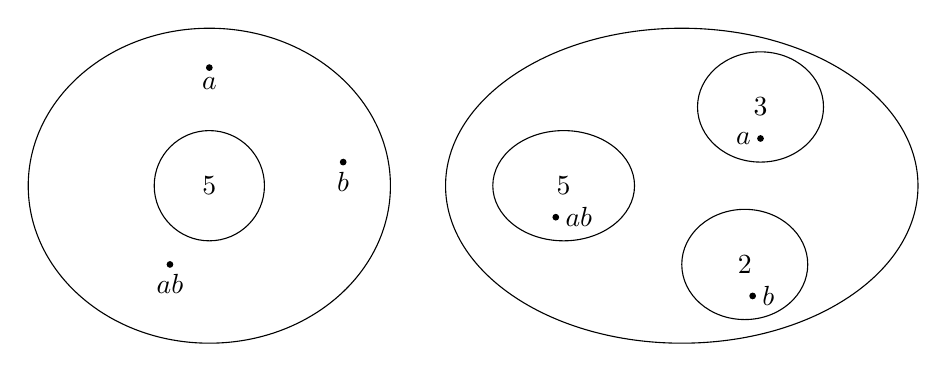
\begin{tikzpicture}
	\filldraw (0,1.5) circle (1pt) node[below] {$a$};
	\filldraw (-.5,-1) circle (1pt) node[below] {$ab$};
	\filldraw (1.7,.3) circle (1pt) node[below] {$b$};
	\node (z5) at (0,0) {$5\Z$};
	
	\draw (z5) ellipse (.7 and .7);
	\draw (z5) ellipse (2.3 and 2);
	
	\begin{scope}[shift={(6,0)}]
	\filldraw (-1.6,-.4) circle (1pt) node[right] {$ab$};
	\filldraw (1,.6) circle (1pt) node[left] {$a$};
	\filldraw (.9,-1.4) circle (1pt) node[right] {$b$};
	\node (z6) at (-1.5,0) {$5\Z$};
	\node (z3) at (1, 1) {$3\Z$};
	\node (z2) at (.8, -1) {$2\Z$};
	\node (op) at (0,0) {};
	
	\draw (z6) ellipse (.9 and .7);
	\draw (z3) ellipse (.8 and .7);
	\draw (z2) ellipse (.8 and .7);
	\draw (op) ellipse (3 and 2);
	\end{scope}
	\end{tikzpicture}
	\caption{Ejemplo de un ideal primo ($5\Z$) y otro no primo ($6\Z$).}
\end{figure}

\begin{ej}
	En $\Z$ el $\{\0\}$ es un ideal primo. También lo es $5\Z$. Por el contrario $6\Z$ no lo es.\footnote{Vaya que chorprecha que los $p\Z$ con $p$ primo sean ideales primos.}
\end{ej}

%TODO probar
\begin{pro}
	Un anillo $A$ es un DI $\iff \{\0\}$ es un ideal primo.
\end{pro}

\subsection{Retículo de ideales. Ideales maximales.}

% TODO
\begin{dfn}[Retículo de ideales]
	Estaría bien tener una definición de esto.
\end{dfn}


\begin{ej}
	En $(\Z/8\Z, +, \cdot)$ el retículo de ideales coincide con los subgrupos de $(\Z/8\Z, +)$:
	\begin{align*}
		\{\overline{0}\} \subset \gen{\overline{4}} = \{\overline{0}, \overline{4}\} \subset \gen{\overline{2}} = \{\overline{0}, \overline{2}, \overline{4}, \overline{6}\} \subset \Z/8\Z
	\end{align*}
\end{ej}

\begin{dfn}[Ideal maximal]
	Sea $I \subsetneq A$ un ideal propio. Diremos que $I$ es un ideal maximal $\iff \forall J$
	\begin{align*}
		J \text{ ideal } \land I \subseteq J \subset A \implies J = I \lor J = A
	\end{align*}
\end{dfn}

\begin{pro}
	En el anillo $(\Z, +, \cdot)$ son ideales maximales $p\Z$ con $p$ primo.
\end{pro}

\begin{figure}[h]
	\centering
	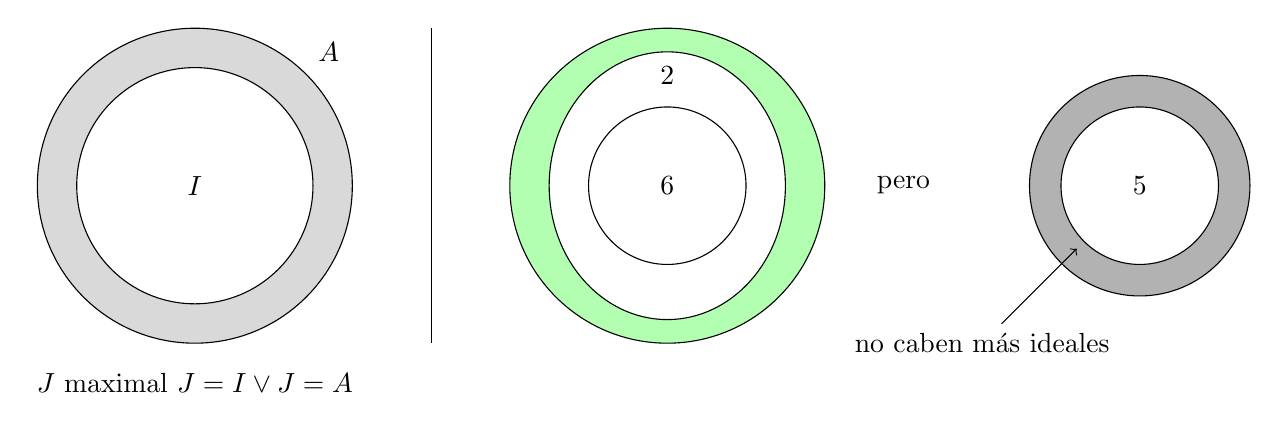
\begin{tikzpicture}
		\draw[black,fill=gray!30] (0,0) ellipse (2 and 2);
		\draw[black,fill=white] (0,0) ellipse (1.5 and 1.5);
		\node (I) at (0,0) {$I$};
		\node (A) at (1.7,1.7) {$A$};
		\node (t) at (0,-2.5) {$J$ maximal $\implies J = I \lor J = A$};
		
		\draw (3,2) -- (3,-2);
		
		\begin{scope}[shift={(6, 0)}]
		\draw[black,fill=green!30] (0,0) ellipse (2 and 2);
		\draw[black,fill=white] (0,0) ellipse (1.5 and 1.7);
		\draw[black,fill=white] (0,0) ellipse (1 and 1);
		\node (6z) at (0,0) {$6\Z$};
		\node (2z) at (0,1.4) {$2\Z$};
		\node (z) at (1.7,1.7) {$\Z$};
		\end{scope}
		
		\node (pero) at (9,0) {pero};
		
		\begin{scope}[shift={(12, 0)}]
		\draw[black,fill=gray!60] (0,0) ellipse (1.4 and 1.4);
		\draw[black,fill=white] (0,0) ellipse (1 and 1);
		\node (5z) at (0,0) {$5\Z$};
		\node (z) at (1.2,1.2) {$\Z$};
		
		\node (nota) at (-2,-2) {no caben más ideales};
		\draw[->] (nota) -- (-0.8, -0.8); 
		\end{scope}
	\end{tikzpicture}
	\caption{Diferencia entre un ideal maximal y uno no maximal. Aquí $6\Z$ no es maximal pero $5\Z$ sí que lo es.}
\end{figure}

\subsection{Relación de equivalencia inducida por los ideales}

\begin{dfn}[Relación de equivalencia por ideales]
	Sea $I \subset A$ un ideal. Definimos la relación de equivalencia $a_1 R a_2 \iff a_1 - a_2 \in I$.
\end{dfn}

\begin{pro}
	$R$ es efectivamente una relación de equivalencia
\end{pro}

\begin{proof}Probamos las 3 propiedades de las relaciones de equivalencia:
	\begin{enumerate}
		\item Reflexiva: $\forall a_1 \in A,\ a_1 - a_1 = \0 \in I \implies a_1Ra_1$
		\item Simétrica: $\forall a_1, a_2 \in A$ con $a_1 R a_2$ tenemos que $a_2 - a_1 = -(a_1 - a_2) \in I \implies a_2 R a_1$
		\item Transitiva: $a_1Ra_2 \land a_2Ra_3 \implies (a_1 - a_2) \in I \land (a_2 - a_3) \in I \implies ((a_1 - a_2) - (a_2 - a_3) \in I \implies (a_1 - a_3) \in I \implies a_1 R a_3$
	\end{enumerate}
\end{proof}

¿Cómo son las clases de equivalencia que viven en el conjunto cociente $A/I$? Pues son de la forma $\overline{a} = a + I = \{a + i_i \mid i_i \in I\}$. Podemos dotar de estructura de anillo a este conjunto cociente. Las operaciones que definimos son las naturales:

\begin{dfn}[Estructura de anillo del cociente]
	Sea $(A, +, \cdot)$ un anillo, $I \subset A$ un ideal. La relación de equivalencia $a_1 R a_2 \iff a_1 - a_2 \in I$ define una partición en clases de equivalencia $\overline{a} \in A/I$. Definimos las operaciones $\#$ y $\bullet$
	
	\begin{align}
		\overline{a} \# \overline{b} = a + i_i + b + i_j = a+b + \underbrace{i_i + i_j}_{\in I} = \overline{a+b} \\
		\overline{a}\bullet\overline{b} = (a+i_i)(b+i_i) = ab + \underbrace{a i_i + b i_j + i_i i_j}_{\in I} = \overline{a \cdot b}
	\end{align}
	De este modo $(A/I, \#, \bullet)$ es un anillo y $\pi: A \to A/I$ definido con $a \mapsto \pi(a) = \overline{a}$ es un homomorfismo de anillos.
\end{dfn}

\begin{pro}
	Lo que dice la definición es verdad: $(A/I, \#, \bullet)$ es un anillo y $\pi$ un homomorfismo de anillos.
\end{pro}

\begin{pro}
	La función $\pi: A \to A/I$ que da las clases de equivalencia es un epimorfismo de grupos (es sobreyectivo) y además $\ker \pi = I$.
\end{pro}

\begin{pro}
	$P \subset A$ ideal primo $\iff A/P$ es un dominio de integridad
\end{pro}

\begin{figure}[h]
	\centering
	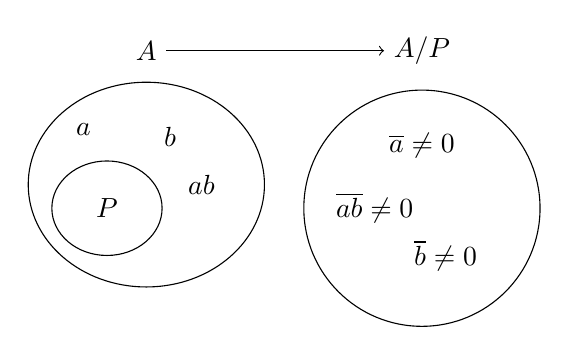
\begin{tikzpicture}
	% TODO: poner puntitos en los nodos
	\node (a) at (-0.3,1) {$a$};
	\node (b) at (0.8,0.9) {$b$};
	\node (ab) at (1.2, .3) {$ab$};
	\node (P) at (0,0) {$P$};
	\node (A) at (0.5,2) {$A$};
	
	\draw (P) ellipse (.7 and .6);
	\draw (0.5,0.3) ellipse (1.5 and 1.3);
	
	\begin{scope}[shift={(4,0)}]
	\node (AP) at (0, 2) {$A/P$};
	\node (abp) at (-.6, 0) {$\overline{ab} \neq 0$};
	\node (ap) at (0, .8) {$\overline{a} \neq 0$};
	\node (bp) at (0.3,-.6) {$\overline{b} \neq 0$};
	\draw (0,0) ellipse (1.5 and 1.5);
	\end{scope}
	\draw[->] (A) -- (AP);
	\end{tikzpicture}
\end{figure}

\begin{proof}
	Sabemos que
	\begin{align*}
		a \notin P &\iff \overline{a} \neq \overline{\0} \text{ en } A/P \\
		b \notin P &\iff \overline{b} \neq \overline{\0} \text{ en } A/P \\
		a\cdot b \notin P &\iff \overline{a\cdot b} = \overline{a}\cdot \overline{b} \neq \overline{\0} \text{ en } A/P
	\end{align*}
	Luego es claro que $P$ ideal primo $\iff$ el producto de elementos no nulos es no nulo en $A/P \iff A/P$ es un DI (dominio de integridad).
\end{proof}

\subsection{Correspondencia entre ideales}

Ahora damos un teorema análogo al de correspondencia que dimos para subgrupos (\autoref{thm:correspondenciasubgrupos}).

\begin{thm}[de correspondencia entre ideales]
	Sea $(A, +, \cdot)$ un anillo, $I \subsetneq A$ un ideal propio de $A$. Sea $\pi: A \to A/I$ la función sobreyectiva que da las clases de equivalencia para cada elemento $a \in A \mapsto \overline{a}$ que tiene $\ker \pi = I$. Se tiene
	\begin{enumerate}
		\item Si $\overline{J}$ es un ideal en $A/I$ entonces $\inv{\pi}(\overline{J})$ es un ideal en $A$ que contiene a $I$
		\item Si $K$ es un ideal en $A$ que contiene a $I$, entonces $K = \inv{\pi(\pi(K))}$, es decir, $K$ es la contraimagen de algún ideal $\pi(K) \subset A/I$.
	\end{enumerate}
\end{thm}

\begin{obs}
	El ideal $\{\overline{\0}\}$ de $A/I$ tiene contraimagen $\inv{\pi}(\{\overline{\0}\}) = I$.
\end{obs}

\begin{obs}
	Si $\overline{J}$ es un ideal en $A/I$.
	
	\begin{figure}[h]
		\centering
		\begin{tikzpicture}
			\node (A) at (0,0) {$A$};
			\node (AI) at (2,0) {$A/I$};
			\node (AIJ) at (2,-2) {$\frac{A/I}{\overline{J}}$};
			
			\draw[->] (A) -- (AI) node[pos=.5, above] {$\pi$};
			\draw[->] (AI) -- (AIJ) node[pos=.5,right] {$\pi'$};
		\end{tikzpicture}
		\caption{Ejemplo de una doble aplicación del teorema de correspondencia.}
	\end{figure}
	La composición $\pi' \circ \pi$ es un homomorfismo de anillos y además $\ker (\pi' \circ \pi) = \inv{\pi}(\overline{J})$
\end{obs}

\begin{ej}[de aplicación del teorema de correspondencia entre ideales para anillos]
	
	Buscamos el retículo de ideales de $\Z/12\Z$. Por alguna razón sabe que el retículo de $\Z/12\Z$ se identifica con el retículo de ideales de $\Z$ que contienen al $6\Z$ así que se define $\pi: \Z \to \Z/12\Z$. Luego afirma que en $\Z/6\Z$ hay exáctamente un ideal por divisor positivo de $6$.
\end{ej}

\begin{pro}
	En $\Z/n\Z$ hay un ideal por cada divisor positivo de $n$.
\end{pro}

\begin{ej}[Retículo de ideales de $(\Z, +, \cdot)$]
	
	Sabemos que los ideales de $\Z$ son de la forma $n\Z = 0\Z, 1\Z, 2\Z, 3\Z, 4\Z, \dots$ para $n = 0,1,2,3,\dots$ Observemos que podemos construir el retículo sabiendo que $n\Z \subset m\Z \iff n \in m\Z\iff m \divides n$. Así nos va quedando el retículo:
	
	\begin{figure}[h]
		\centering
		% TODO sombrear los que contienen al 6
		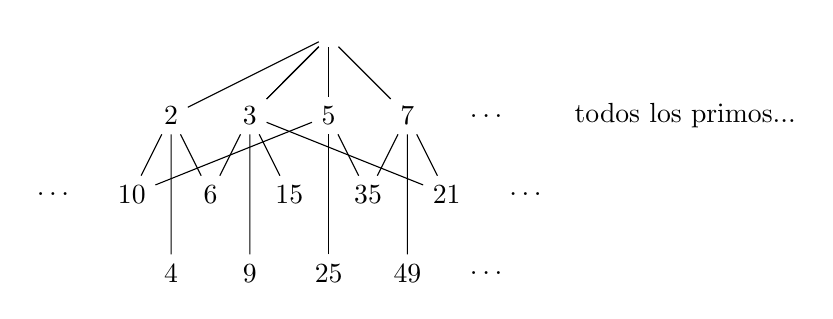
\begin{tikzpicture}
			\node (z) at (0,1) {$\Z$};
			\node (2z) at (-2,0) {$2\Z$};
			\node (3z) at (-1,0) {$3\Z$};
			\node (5z) at (0,0) {$5\Z$};
			\node (7z) at (1,0) {$7\Z$};
			\node (dots) at (2,0) {$\dots$};
			\node[right] (prims) at (3,0) {todos los primos...};
			
			\node (mmdots) at (-3.5,-1) {$\dots$};
			\node (10z) at (-2.5,-1) {$10\Z$};
			\node (6z) at (-1.5,-1) {$6\Z$};
			\node (15z) at (-0.5,-1) {$15\Z$};
			\node (35z) at (0.5,-1) {$35\Z$};
			\node (21z) at (1.5, -1) {$21\Z$};
			\node at (2.5, -1) {$\dots$};
			
			\node (4z) at (-2,-2) {$4\Z$};
			\node (9z) at (-1, -2) {$9\Z$};
			\node (25z) at (0,-2) {$25\Z$};
			\node (49z) at (1, -2) {$49\Z$};
			\node at (2,-2) {$\dots$};
			
			\draw 	(4z) -- (2z)
					(2z) -- (z);
			\draw 	(9z) -- (3z)
					(3z) -- (z);
			\draw 	(25z) -- (5z)
					(5z) -- (z);
			\draw 	(49z) -- (7z)
					(7z) -- (z);
			\draw	(10z) -- (2z)
					(10z) -- (5z);
			\draw 	(6z) -- (2z)
					(6z) -- (3z);
			\draw	(15z) -- (3z)
					(3z) -- (z);
			\draw	(35z) -- (5z)
					(35z) -- (7z);
			\draw	(21z) -- (3z)
					(21z) -- (7z);
		\end{tikzpicture}
		\caption{Retículo de ideales de $(\Z, +, \cdot)$.}
	\end{figure}
\end{ej}

\section{Producto directo}

\subsection{Producto directo en anillos}

\begin{dfn}[Producto directo en anillos]
	Sean $(A, +_A, \cdot_A), (B, +_B, \cdot_B)$ dos anillos con unidad. Definimos el producto directo $A \times B$ como el anillo $(A \times B, \#, \bullet)$ donde las operaciones se definen:
	\begin{align*}
		\# : (A\times B) \times (A\times B) \to A \times B\qquad &(a_1, b_1) \# (a_2, b_2) = (a_1 +_A a_2, b_1 +_B b_2) \\
		\bullet : (A\times B) \times (A\times B) \to A \times B\qquad &(a_1, b_1) \bullet (a_2, b_2) = (a_1 \cdot_A a_2, b_1 \cdot_B b_2)
	\end{align*}
\end{dfn}

\begin{pro}
	$(A\times B, \#, \bullet)$ en efecto es un anillo.
\end{pro}

\begin{obs}
	En el nuevo anillo $(A\times B, \#, \bullet)$ el elemento neutro aditivo es $\0_{A\times B} = (\0_A, \0_B)$ y el elemento neutro multiplicativo es $(\1_A, \1_B)$.
\end{obs}

\begin{pro}
	$(a,b) \in \uds{A \times B} \iff a \in \uds{A} \land b \in \uds{B}$
\end{pro}

\begin{proof}
	$(a,b) \in \uds{A \times B} \iff \exists (a',b') \in A\times B \mid (a,b) \bullet (a', b') = (\1_A, \1_B) \iff a\cdot_A a' = \1_A \land b\cdot_B b' = \1_B \iff a \in \uds{A} \land b \in \uds{B}$
\end{proof}

\begin{ej}
	Las unidades de $\Z \times \Z$ son
	\begin{align*}
		\uds{\Z \times \Z} = (\{(1,1), (1,-1), (-1,1), (-1,-1)\}, \bullet)
	\end{align*}
\end{ej}

\begin{ej}
	Sea $s \in A,\ s\neq \0$. Fijado $s$, definimos $\alpha_s : A \to A, a \mapsto a\cdot s$. Observemos:
	\begin{enumerate}
		\item $\alpha_s$ es un homomorfismo de grupos
		\item $\alpha_s$ es inyectivo $\iff \ker \alpha_s = \{ \0 \}$
		\begin{itemize}
			\item $\ker \alpha_s = \{\0\} \iff s$ no es divisor de $\0$
			\item $\ker \alpha_s \neq \{\0\} \iff s$ es divisor de $\0$
		\end{itemize}
		\item $\ima \alpha_s = \gen{\{s\}}$
		\begin{itemize}
			\item $s \in \uds{A} \iff \gen{s}$ (ver \autoref{pro:inunidadesiffgenerado}), por tanto $\alpha_s$ es sobre $\iff \ima \alpha_s = A \iff \gen{s} = A \iff s \in \uds{A}$.
		\end{itemize}
		
	\end{enumerate}
\end{ej}

Este ejemplo nos permite dar el siguiente teorema:

\begin{thm}
	Sea $(A, +, \cdot)$ un anillo finito y sea $a \in A \setminus \{\0\}$. Entonces, o bien $a \in \uds{A}$, o bien $a$ es un divisor de $\0$. Por tanto escribimos
	\begin{align*}
	A \setminus \{\0\} = \uds{A} \bigcup_{\text{disjunta}} \{a \in A \mid a \text{ divisor de }\0\}
	\end{align*}
\end{thm}

\begin{proof}
	Fijo $s \in A \setminus \{\0\}$. Como $A$ es finito $\alpha_s$ inyectiva $\iff \alpha_s$ sobreyectiva $\iff \alpha_s$ inyectiva. Entonces, fijándonos en el ejemplo anterior, tenemos
	\begin{itemize}
		\item Si $s \in \uds{A}$ entonces $\alpha_s$ inyectiva $\implies \ker \alpha_s = \{\0\} \implies s$ no es un divisor de $0$.
		\item Si $s \notin \uds{A}$ entonces $\alpha$ no es sobre $\implies \alpha_s$ no inyectiva $\implies \ker \alpha_s \neq \{\0\} \implies s$ es un divisor de $\0$.
	\end{itemize}
\end{proof}

\begin{ej}
	Sea $A = \Z/8\Z \times \Z/10\Z$. ¿Cuántos divisores de $\0$ tiene $A$?
\end{ej}

\begin{proof}
	Sabemos que $|A| = 80 \implies A \setminus \{\0\}$ tiene 79 elementos. Además sabemos que $\uds{A} = \uds{\Z/8\Z} \times \uds{\Z/10\Z} \implies |\uds{A}| = 4 \times 4 = 16$. Luego hay $79 - 16 = 63$ divisores de $\0$ en $A$.
\end{proof}

\begin{ej}
	Sabemos que en $\Z$ todo $n\Z$ es un ideal. ¿Ocurre lo mismo para $\{(n,n) \mid n \in \Z\} \subset \Z \times \Z$? La respuesta es que NO. Contraejemplo: $(\1,\0) \bullet (3,3) = (3,\0) \notin \{(n,n) \mid n \in \Z\}$ (al no ser cerrado por el producto no es un subanillo y por tanto tampoco es un ideal).
\end{ej}

\subsection{Producto directo en cuerpos}

Nos preguntamos ahora: ¿Si $A, B$ son cuerpos, es $A \times B$ un cuerpo? La respuesta es que NO. Contraejemplo:
\begin{align*}
	\underbrace{(\1_A,\0_B)}_{\neq (\0_A, \0_B)} \bullet (a,b) = (\1_A, \1_B) \iff \begin{cases}
	\1_A \cdot_A a = \1_A \\
	\0_B \cdot_B b = \1_B \longrightarrow\text{ sin solución }
	\end{cases}
\end{align*}


%-------------------------
%-------------------------
%-------------------------
\section{Por revisar}

% -------------

\begin{thm}
	Dado el anillo $A$ y un ideal propio $I$
	\begin{align*}
		\pi: A \to A/I,\qquad I \subset \inv{\pi}(\overline{J}) \subset A,\qquad \overline{0} \in \overline{J} \subset A / I
	\end{align*}
	
	existe una identificación entre el retículo de ideales $A / I$ con el subretículo de ideales de $A$ que contienen a $I$. 
	
	Es decir, si $J$ es un ideale en $A/I$ entonces $\inv{\pi}(\overline{J})$ es un ideal en $A$ que contiene al ideal $I$.
\end{thm}


El ideal cero de $A/I$ tiene contraimagen $\inv{\pi}(\{0\}) = I$. Si $\overline{J}$ es un ideal en $A/I$
\begin{align*}
	\pi : A \to A/I \to (A/I) / \overline{J}
\end{align*}

es un homomorfismo de anillos (la composición de homomorfismos de anillos es un homomorfismo de anillos). $\inv{\pi}(\overline{J}) = \ker$ de la composición.

% --------------------

\begin{thm}
	Sea $\alpha: A \to B$ un homomorfismo de anillos.
	\begin{itemize}
		\item $\ker \alpha$ es un ideal
		\item $\ima \alpha$ es un subanillo
		\item $\alpha$ es sobreyectivo $\iff \ima \alpha = B$
		\item $\alpha$ es inyectivo $\iff \ker \alpha = \{\0\}$
	\end{itemize}
\end{thm}

\begin{dfn}[Isomorfismo de anillos]
	Un homomorfismo de anillos $\alpha: A \to B$ es un isomorfismo cuando es una biyección. En este caso decimos que $A$ y $B$ son isomorfos y lo notamos con $A \isom B$.
\end{dfn}

\begin{pro}
	Si $\alpha: A \to B$ es un homomorfismo de anillos y una biyección de conjuntos entonces $\inv{\alpha}:B \to A$ es nuevamente un homomorfismo de anillos.
\end{pro}

\subsubsection{Homomorfismos de anillos e ideales}

\begin{thm}
	Sea $\alpha: A \to B$ un homorfismo de anillos. Entonces
	\begin{enumerate}
		\item Si $J \subset B$ es un ideal en $B$ entonces $\inv{\alpha}(J)$ es un ideal en $A$.
		\item Si $\alpha$ es sobreyectiva entonces la imagen $\alpha(I)$ de un ideal $I \subset A$ es un ideal en $B$
	\end{enumerate}
\end{thm}

\begin{proof}
	\begin{figure}[h]
		\centering
		\begin{tikzpicture}
		\node (A) at (0,0) {$A$};
		\node (B) at (4,0) {$B$};
		\node (BJ) at (4, -3) {$B / J$};
		
		\draw[-{Latex[length=2mm]}] (A) -- (B) node[pos=.5, above] {$\alpha$};
		\draw[-{Latex[length=2mm]}] (B) -- (BJ) node[pos=.5, left]{$\pi$};
		\draw[-{Latex[length=2mm]}] (A) -- (BJ) node[pos=.5, below] {$\pi \circ \alpha$};
		\end{tikzpicture}
	\end{figure}
	\begin{enumerate}
		\item $\inv{\alpha}(J) = \ker(\pi \circ \alpha)$ y por tanto es un ideal.
		\item Probamos las propiedades de los ideales:
		\begin{enumerate}
			\item $\alpha(0) = 0 \in \alpha(I)$
			\item Sean $b_1, b_2 \in \alpha(I)$ tenemos que ver que $b_1 + b_2 \in \alpha(I)$. Sean $a_1, a_2 \in I$ tales que $b_1 = \alpha(a_1) \land b_2 = \alpha(a_2)$. Por ser $\alpha$ h. de anillos tenemos que $b_1 + b_2 = \alpha(a_1 + a_2) = \alpha(a_1) + \alpha(a_2)$.
			\item Sean $b \in B,\ b' \in \alpha(I)$. Tenemos que probar que $bb' \in \alpha(I)$. Sabemos que $b' \in \alpha(I) \iff b' = \alpha(a),\ a \in I$. Como $b \in B$ y $\alpha$ es sobre tiene que existir $d \in I \mid \alpha(d) = b$. Por tanto $\alpha(d\cdot a) = b \cdot b' \implies bb' \in \alpha(I)$.
		\end{enumerate}
	\end{enumerate}
\end{proof}

Fijado $I \subset A$ consideramos $\pi:A \to A/I$ que es un homomorfismo de anillos sobreyectivo.

\begin{enumerate}
	\item Si $\overline{J} \subset A /I$ es un ideal en $A / I$ entonces $\inv{\pi}(\overline{J})$ es un ideal en $A$ que contiene a $I$.
	\item Si $J$ es un ideal en $A$ entonces $\pi(J)$ es un ideal en $A/J$ y $J \subseteq \inv{\pi}(\pi(J))$ (es claro porque si $j \in J$ entonces $\pi(j) \in \pi(J)$).
	\begin{enumerate}
		\item Además, si $I \subseteq J$ entonces $J = \inv{\pi}(\pi(J))$.
		\begin{proof}
			Si $\delta \in \inv{\pi}(\pi(J)) \implies \delta \in J$. Además, $\delta \in \inv{\pi}(\pi(J)) \iff \pi(\delta) \in \pi(J) \iff \pi(\delta) = \pi(d_1),\ d_1 \in J \iff \delta - d_1 \in \ker \pi = I$. Tomamos
			\begin{align*}
				\delta = \underbrace{(\delta - j_i)}_{\in I} + \underbrace{j_i}_{\in J} \in J
			\end{align*}
			porque $I \subset J$.
		\end{proof}
	\end{enumerate}
\end{enumerate}


La siguiente proposición nos llevará al primer teorema de la isomorfía.
\begin{pro}
	Sea $\varphi: A \to B$ un homomorfismo de anillos con $\ker \varphi$ ideal en $A$. Sea $I$ un ideal en $A$ con $I \subset \ker \varphi$.
	\begin{itemize}
		\item Existe un único homomorfismo de anillos $\overline{\varphi}: A / I \to B$ tal que $\varphi = \overline{\varphi} \circ \pi$.
		\begin{figure}[h]
			\centering
			\begin{tikzpicture}
			\node (A) at (0,0) {$A$};
			\node (B) at (4,0) {$B$};
			\node (AI) at (0, -3) {$A / I$};
			
			\draw[-{Latex[length=2mm]}] (A) -- (B) node[pos=.5, above] {$\varphi$};
			\draw[-{Latex[length=2mm]}] (A) -- (AI) node[pos=.5, left]{$\pi$};
			\draw[-{Latex[length=2mm]}] (AI) -- (B) node[pos=.5, below] {$\overline{\varphi}$};
			\end{tikzpicture}
		\end{figure}
		\begin{proof}
			Definimos $\overline{\varphi}(\overline{a}) = \varphi(a)$. Aunque choque (porque el $\overline{a}$ puede venir de muchos $a$) aseguramos que $\overline{\varphi}$ está bien definida. Veamos por qué. Sabemos que $a'$ y $a$ definen el mismo elemento en $A / I \iff a' - a \in I$. Sopongamos que $I \subset \ker \varphi$. Entonces $\varphi(a - a') = 0 \iff \varphi(a) - \varphi(a') = 0 \implies \overline{\varphi}$ está bien definida como función.
			
			Veamos ahora que en efecto se cumple que $\overline{\varphi}$ es un homomorfismo de anillos, es decir que $\overline{\varphi}(\overline{a} + \overline{b}) = \overline{\varphi}(\overline{a}) + \overline{\varphi}(\overline{b})$. Recordando la definición que hemos dado de $\varphi$ y la propiedad $\overline{a} + \overline{b} = \overline{a + b}$ es claro que $\overline{\varphi}(\overline{a} + \overline{b}) = \overline{\varphi}(\overline{a +b}) = \varphi(a + b) = \varphi(a) + \varphi(b) = \overline{\varphi}(\overline{a}) + \overline{\varphi}(\overline{b})$. Es análogo para el producto ya que $\overline{a} \cdot \overline{b} = \overline{a \cdot b}$.
		\end{proof}
		\item $\ker \overline{\varphi} = \ker \varphi / I$
		\begin{proof}
			Sea $\overline{a} \in A / I$. Entonces $\overline{a} \in \ker \overline{\varphi} \iff \overline{\varphi}(\overline{a}) = 0 \iff \varphi(a) = 0 \iff a \in \ker \varphi$.
		\end{proof}
	\end{itemize}
\end{pro}

\begin{thm}[Primer teorema de la isomorfía (anillos)]
	Si $\alpha: A \to B$ es un homomorfismo de anillos sobreyectivo entonces $B \isom A / \ker \alpha$.
\end{thm}

	\begin{figure}[h]
	\centering
	\begin{tikzpicture}
	\node (A) at (0,0) {$A$};
	\node (B) at (4,0) {$B$};
	\node (AI) at (0, -3) {$A / \ker \alpha$};
	
	\draw[-{Latex[length=2mm]}] (A) -- (B) node[pos=.5, above] {$\alpha$};
	\draw[-{Latex[length=2mm]}] (A) -- (AI) node[pos=.5, left]{$\pi$};
	\draw[-{Latex[length=2mm]}] (AI) -- (B) node[pos=.5, below] {$\overline{\alpha}$};
	\end{tikzpicture}
\end{figure}

\begin{proof}
	Nos apoyamos en la proposición anterior tomando $I = \ker \alpha$. Como $\alpha$ y $\pi$ son sobreyectivas tenemos que $\overline{\alpha}$ es sobreyectiva. Aplicando el segundo resultado de la proposición anterior tenemos que $\ker \overline{\alpha} = \ker \alpha / \ker \alpha = \{ 0\} \implies \overline{\alpha}$ es inyectiva. Concluimos que $\overline{\alpha}$ es un isomorfismo de anillos y por tanto $B \isom A / \ker \alpha$.
\end{proof}

% ------- 20181217

\begin{thm}
	\begin{align*}
	D \text{ es un dominio de ideales principales (DIP) } \implies D \text{ es un dominio de factorización única (DFU)}
	\end{align*}
\end{thm}

El recíproco de este teorema no es cierto en general. Véase por ejemplo el caso de $\Z$ que es un dominio de ideales principales pero no se cumple que $\Z[X]$ es un dominio de factorización única. Si se cumpliera el recíproco entonces el siguiente teorema sería un simple corolario.

\begin{thm}
	\begin{align*}
	D \text{ es un dominio de factorización única (DFU) } \implies D[X] \text{ es un dominio de factorización única (DFU)}
	\end{align*}
\end{thm}

Este segundo teorema no lo vamos a probar. Probamos el primero.

\begin{dfn}[Asociados]
	Sea $D$ un domino, $a,a' \in D$. DIremos que $a$ y $a'$ son asociados $\iff \exists u \in \uds{D} \mid a = u a'$.
\end{dfn}

\begin{proof}
	Sea $D$ un dominio, $a \in D \mid a \neq 0 \land a \not\in \uds{D}$. Sabemos que $a, a' \in D$ son asociados si $\exists u \in \uds{D} \mid a = ua'$. Por ejemplo, los polinomios $3x-2$ y $x - 2/3$ en $\Q[X]$ son asociados.
	
	Observemos que si $a$ y $a'$ son asociados entonces $\gen{a} = \gen{a'}$. Si $u \in \uds{a}$ entonces $ua' = a \in \gen{a'}$. Análogamente $\inv{u}a = a' \in \uds{a}$. Luego tenemos $\gen{a} \subset \gen{a'} \land \gen{a'} \subset \gen{a} \implies \gen{a} = \gen{a'}$. Recíprocamente si $0 \neq \gen{a} = \gen{a'} \implies \exists u \in \uds{D} \mid a = ua'$. $a \in \gen{a'} \land a' \in \gen{a} \implies a = a't \land a' = as \implies a' = a'ts \implies 1 = ts \implies t,s \in \uds{D}$.
	
	Recordemos las hipótesis iniciales: $a \in D \mid a \neq 0 \land a \not\in \uds{D}$. Esto nos da que $0 \neq \gen{a} \land \gen{a} \subsetneq D$. Pensemos en qué significa que un elemento no nulo $a$ no sea una unidad. Supongamos $a = st$. Si $a$ no es una unidad podría ocurrir que $s$ es una unidad (por ejemplo $6 = (-1)(-6),\ -1 \in \uds{\Z}$). Lo que sí que está claro es que no puede ocurrir que a la vez $s$ y $t$ sean unidades. Es decir, tiene que ocurrir que al menos uno de los dos no es una unidad. Por tanto podemos suponer sin pérdida de generalidad que si expresamos $a = a' \cdot s$  entonces $a' \not \in \uds{D}$. Tenemos dos situaciones posibles
	\begin{enumerate}
		\item $s \in \uds{D} \implies \gen{a} = \gen{a'}$
		\item $s \not \in \uds{D} \implies \gen{a} \subsetneq \gen{a'}$ ya que $\gen{a} = \gen{a'} \iff a = a'u$ con $u \in \uds{D}$ pero hemos tomado $s \not\in \uds{D}$
	\end{enumerate}
\end{proof}

Aquí para de demostrar y empieza a dar definiciones.

\begin{dfn}[Irreducible]
	Sea $D$ un dominio y $0 \neq a \not\in \uds{D}$. Diremos que $a$ es irreducible en $D \iff \forall a',s \in D,\ a' \not \in \uds{D},\ a = a's \implies s \in \uds{D}$
\end{dfn}

\begin{obs}
	Un elemento es irreducible $\iff$ cualquier asociado lo es.
\end{obs}

\begin{dfn}[Dominio de factorización única (DFU)]
	Sea $D$ un dominio. Diremos que $D$ es un dominio de factorización única (DFU) si se cumplen las siguientes condiciones $\forall a \in D$:
	\begin{itemize}
		\item $a \neq 0 \land a \not\in\uds{D} \implies a = p_1p_2\dots p_r$ donde $p_i$ es irreducible en $D$
		\item $a = p_1p_2\dots p_r,\ p_i$ irreducible y $a = q_1q_2 \dots q_s,\ q_i$ irreducible $\implies r = s$ y además $r_i$ y $q_i$ son asociados para $i = 1, \dots, r$ (la igualdad es un caso particular de el ser asociados).
	\end{itemize}
\end{dfn}

\begin{obs}
	Sea $I_1 \subseteq I_2 \subseteq I_3 \subseteq ...$ una cadena creaciente de ideales de un anillo $A$. Entonces $\bigcup I_i$ es un ideal.\footnote{Literalmente ha dicho que esto no viene a cuento. Que esto es una digresión de las suyas.}
\end{obs}

\begin{proof}
	Probamos las propiedades de los ideales.
	\begin{enumerate}
		\item $0 \in \bigcup I_i$
		\item $s,t \in \bigcup I_i \implies s+t \in \bigcap I_i$
		\item $s \in \bigcup I_i,\ a \in A \implies as \in \bigcup I_i$.
	\end{enumerate}
\end{proof}

\begin{dfn}
	[Propiedad de cadena creciente]
	
	Diremos que un anillo $A$ tiene la propiedad de cadena creciente $\iff$ toda cadena creciente $I_1 \subseteq I_2 \subseteq I_3 \subseteq \dots \subseteq I_n \subseteq \dots$ es finita. Es decir, que $\exists n \mid I_n = I_{n+1} = I_{n+2} = \dots$.
\end{dfn}

\begin{thm}
	Si $D$ es un DIP entonces $D$ tiene la propiedad de cadena creciente.
\end{thm}

La demostración es tan ingenua como uno quiera.

\begin{proof}
	Sea $I_1 \subseteq I_2 \subseteq I_3 \subseteq \dots \subseteq I_n \subseteq \dots$ una cadena de ideales. Sabemos que en cualquier anillo $\bigcup I_i$ es un ideal. Sea $J = \gen{d}$ para algún $d \in D$. Como $D$ es un DIP ocurre que $d \in \bigcup I_i \implies d \in I_{n_0} \implies \gen{d} \subset I_{n_0} \implies I_{n_0} = I_{n_0 + 1} = \dots$
\end{proof}

